\chapter{Návrh aplikace}

Tato kapitola se zabývá návrhem mobilní aplikace na základě výsledků provedené analýzy.
Cílem návrhu je definovat funkční rozsah aplikace, její strukturu, uživatelské rozhraní a technologické řešení tak, aby odpovídaly potřebám cílových uživatelů a zvolenému zaměření aplikace.
K tomuto byly využity standardní techniky softwarového inženýrství, zejména
specifikace požadavků a návrhové diagramy.

Nejprve jsou specifikovány funkční a nefunkční požadavky, které vymezují chování a vlastnosti aplikace.
Na jejich základě je dále vytvořen use case diagram znázorňující základní interakce mezi uživateli a aplikací.
Struktura aplikace je následně popsána pomocí class diagramu, který zachycuje hlavní entity a jejich vzájemné vztahy.
Součástí kapitoly je také návrh uživatelského rozhraní, jenž se zaměřuje na rozvržení obrazovek a způsob interakce s~uživatelem.
Závěrečná část kapitoly se věnuje výběru technologií, které budou vyhovovat požadavkům aplikace a umožní její efektivní implementaci.


\section{Specifikace požadavků}

Tato kapitola se zabývá specifikací požadavků na navrhovanou aplikaci.
Požadavky vymezují očekávané chování systému a jeho vlastnosti z pohledu uživatelů i provozu aplikace.

\subsection{Funkční požadavky}

Funkční požadavky popisují chování aplikace a funkce, které aplikace poskytuje svým uživatelům.
Aplikace rozlišuje dva základní typy uživatelů – běžné návštěvníky aplikace a registrované uživatele.

\begin{itemize}
    \item Uživatel může zobrazit obchody v~mapovém nebo seznamovém zobrazení.
    \item Uživatel může filtrovat zobrazené obchody podle kategorie, vzdálenosti a průměrného hodnocení.
    \item Uživatel může zobrazit detail obchodu, včetně popisu, fotografií a kontaktních údajů.
    \item Uživatel může vytvořit uživatelský účet.
    \item Registrovaný uživatel může vytvářet nové obchody.
    \item Registrovaný uživatel může upravovat a spravovat obchody, které vytvořil.
    \item Registrovaný uživatel může upravovat své kontaktní údaje zobrazované u~jeho obchodů.
    \item Registrovaný uživatel může ke svým obchodům přidávat název, popis, kategorie nabízených produktů, fotografie, nabídku produktů a otevírací dobu.
    \item Registrovaný uživatel může vytvářet recenze obchodů ostatních uživatelů.
\end{itemize}

Aplikace neslouží jako e-shop a neumožňuje přímý nákup nebo objednávky.
Jejím cílem je poskytnout prostředek pro prezentaci nabídky domácích producentů na mapě a umožnit zájemcům snadno vyhledat obchody v~jejich okolí.

\subsection{Nefunkční požadavky}

Nefunkční požadavky popisují vlastnosti aplikace, které se netýkají přímo funkcionality, ale ovlivňují kvalitu, použitelnost a provoz aplikace.

\begin{itemize}
    \item Aplikace je určena pro platformu Android.
    \item Uživatelské rozhraní aplikace musí být přehledné a snadno použitelné i~pro méně technicky zdatné uživatele.
    \item Aplikace musí umožňovat plynulé zobrazení mapy a obchodů bez výrazných prodlev.
    \item Data uložená v~aplikaci musí být přístupná pouze oprávněným uživatelům.
    \item Aplikace musí být navržena tak, aby bylo možné ji dále rozšiřovat o~další funkce.
\end{itemize}


\section{Use case diagram}
% TODO: Spis by se hodilo cesky Diagranm pripadu uziti. podobne nasledujici kapitola Diagram trid - jedna se o zazite ceske terminy.
Use case diagram slouží k~přehlednému znázornění základních funkcí aplikace a interakcí mezi uživateli a systémem.
Diagram vychází ze specifikace funkčních požadavků a zachycuje chování aplikace z~pohledu jednotlivých typů uživatelů.
Přehled aktérů a případů užití aplikace je znázorněn na obrázku~\ref{fig:use-case-diagram}.

V~rámci aplikace jsou rozlišeny tři základní role: obecného uživatele (User), zákazníka (Customer) a prodejce (Seller).
Obecný uživatel představuje nadřazenou roli, ze které vycházejí specializované role zákazníka a prodejce.
Tyto specializované role jsou rozděleny podle toho, jakým způsobem chce uživatel aplikaci využívat.

Obecný uživatel zahrnuje možnosti registrace, přihlášení a odhlášení z~aplikace, které jsou přístupné všem uživatelům bez ohledu na jejich způsob využití aplikace.
Umožňuje také úpravu osobních údajů.
Tato možnost je přístupná jakémukoli přihlášenému uživateli.

Zákazník může procházet obchody v~mapovém nebo seznamovém zobrazení, zobrazovat detail obchodu a filtrovat obchody podle kategorií, vzdálenosti nebo hodnocení.
Tyto filtry jsou v~diagramu modelovány jako rozšiřující případy užití nad základními způsoby procházení obchodů.
Pokud je běžný uživatel přihlášen, může vytvářet recenze obchodů ostatních uživatelů.

Třetím aktérem je prodejce, který může vytvářet, upravovat a odstraňovat své obchody.
V rámci správy obchodu může prodejce upravovat polohu obchodu na mapě, otevírací dobu, nabídku produktů a kategorie nabízených produktů.
Všechny interakce prodejce vyžadují přihlášení.

\begin{figure}[h] % [p] pro full page, [h] pro here
    \centering
    \includegraphics[width=\textwidth]{res/use_case_diagram}
    \caption{Use case diagram aplikace}
    \label{fig:use-case-diagram}
\end{figure}
\FloatBarrier


\section{Class diagram}

Class diagram popisuje strukturu aplikace z~pohledu hlavních entit, jejich atributů a vztahů mezi nimi.
Diagram vychází ze specifikace funkčních požadavků a use case diagramu a slouží jako podklad pro návrh datového modelu a implementaci aplikační logiky.
Modeluje základní entity tak, aby systém mohl plnit požadované funkce, zajišťoval konzistenci dat a umožňoval jejich efektivní správu do budoucna.
Přehled hlavních tříd a jejich vztahů je znázorněn na obrázku~\ref{fig:class-diagram}.

Jednou ze základních entit je uživatel (User), který reprezentuje registrovaného uživatele aplikace.
Uživatel je identifikován jednoznačným identifikátorem a obsahuje základní osobní údaje, profilový obrázek a kontaktní informace.
Identifikátor je typu UUID, což zajišťuje jeho jedinečnost napříč celým systémem.
Kontaktní údaje jsou modelovány samostatnou třídou \texttt{ContactInfo}, která je s uživatelem svázána kompozicí, jelikož bez existence uživatele nemají samostatný význam.
Profilový obrázek je volitelný a je reprezentován hodnotovým objektem \texttt{ImageResource}, který uchovává odkaz na externě uložený obrazový soubor.

Druhou klíčovou entitou je obchod (Shop), který reprezentuje obchod vytvořený registrovaným uživatelem, kde může nabízet své produkty.
Obchod je také identifikován jednoznačným identifikátorem typu UUID\@.
Obchod obsahuje atributy: id, název, popis, vlastník, seznam kategorií, obrázky, nabídku produktů, polohu a otevírací dobu.
Základní atributy jako název a popis jsou oba typu \texttt{String} a jsou volitelné.
Obchod je svázán s uživatelem prostřednictvím asociace, která vyjadřuje vlastnictví obchodu konkrétním uživatelem.
Kategorie obchodu je reprezentována hodnotovým objektem \texttt{ShopCategory}, který obsahuje název kategorie a barvu pro vizuální odlišení.
Vztah mezi obchodem a kategoriemi je modelován jako kompozice, protože kategorie jsou vlastněny konkrétním obchodem.
Zakladatel obchodu si tak může zvolit libovolnou kombinaci názvu a barvy pro každou kategorii.
Požadované filtrování obchodů podle kategorií bude realizováno pomocí normalizovaných názvů kategorií ze všech obchodů.
Obrázky obchodu jsou reprezentovány jako seznam již zmiňovaných hodnotových objektů \texttt{ImageResource}.
Nabídka produktů je modelována hodnotovým objektem \texttt{Menu}, který obsahuje seznam položek nabídky typu \texttt{MenuItem}.
Každá položka nabídky obsahuje název, volitelný popis, cenu a informaci o dostupnosti.
Cena je reprezentována hodnotovým objektem \texttt{PriceLabel}, který uchovává cenu jako formátovaný řetězec.
Uživatel tak může cenu popsat vzhledem k měně a jednotce v jaké se produkt nabízí (například \enquote{150 Kč / kg}).
Otevírací doba obchodu je reprezentována rozhraním \texttt{OpeningHours}, které má dvě implementace: \texttt{TimeOpeningHours} a \texttt{MessageOpeningHours}.
První implementace uchovává otevírací dobu jako mapu dnů v týdnu na otevírací hodiny v případě, že producent je dostupný v pravidelných časech.
Druhá implementace uchovává otevírací dobu jako volitelnou zprávu v~případě, že producent chce například uvést, aby ho zájemce nejdříve kontaktoval.
Poloha obchodu je modelována hodnotovým objektem \texttt{Location}, který obsahuje zeměpisnou šířku a délku jako desetinná čísla.

Poslední entitou je recenze (Review), která reprezentuje hodnocení obchodu uživatelem.
Recenze je identifikována jednoznačným identifikátorem typu UUID a obsahuje atributy: id, autor, obchod, hodnocení a volitelný komentář.
Recenze je svázána s uživatelem prostřednictvím asociace, která vyjadřuje autora recenze.
S obchodem je recenze rovněž svázána asociací, jelikož recenze reprezentuje interakci mezi uživatelem a konkrétním obchodem, nikoli jeho vnitřní součást.
Přestože recenze bez existence obchodu ztrácí svůj praktický význam, není modelována jako kompozitní součást obchodu, protože má vlastní identitu a samostatný životní cyklus.

\begin{figure}[p]
    \centering
    \includegraphics[width=\textwidth]{res/class_diagram}
    \caption{Class diagram aplikace}
    \label{fig:class-diagram}
\end{figure}


\section{Návrh uživatelského rozhraní}
% TODO: Jak a na kolika ruznych lidech planujete testovat kvalitu UI?

Návrh uživatelského rozhraní (UI) se zaměřuje na vytvoření přehledného a intuitivního prostředí pro uživatele aplikace.
Cílem je zajistit, aby uživatelé mohli snadno a efektivně využívat funkce aplikace a dosahovat svých cílů, které vychází z funkčních požadavků a use case diagramu.
Návrh UI zahrnuje rozvržení obrazovek, navigační strukturu a interakční prvky.
Při návrhu rozhraní je kladen důraz na konzistenci ovládacích prvků, díky čemuž se uživatel snadno zorientuje v aplikaci, jasnou navigaci aplikací a minimalizaci počtu kroků potřebných k~provedení akcí.

\subsection{Barevné schéma}
% TODO: Co je to material design? Odkaz do literatury!
% TODO: #Material theme builder je v praci navrzen nebo prevzat. V 1. pripade je vhodne odkazat odpovidajici cat text ve durhem zdroj, odkud cerpate.

Aplikace využívá principy Material Designu, které zajišťují jednotný a moderní vzhled aplikace.
Barevná paleta byla vygenerována pomocí nástroje Material Theme Builder, který pomocí jedné primární barvy vytvoří kompletní sadu barev pro světlé i tmavé téma aplikace.
V případě potřeby lze barvy dále upravovat, avšak pro základní návrh zajišťují tyto vygenerované barvy konzistentní a esteticky příjemný vzhled aplikace.
Pro primární barvu byla zvolena tmavě zelená (\#3C6838), která evokuje přírodní potraviny a zemědělství.
Ostatní barvy byly nástrojem Material Theme Builder vygenerovány na základě této primární barvy, aby se vzájemně doplňovaly.
Zajišťují tak dostatečný kontrast pro čitelnost textu a vizuální přitažlivost aplikace.

Významnou barvou v Material Design paletě je barva \textit{surface}, která je používána jako pozadí pro většinu obrazovek aplikace (v obrázku~\ref{fig:color-palette} je použita jako pozadí boxu \enquote{Světlý motiv}, respektive \enquote{Tmavý motiv}).
Těmi nejdůležitějšími barvami jsou ale barvy primární, sekundární, terciární a jejich kontejnerové varianty (zobrazeny na~obrázku~\ref{fig:color-palette}).
Primární, sekundární a terciární barvy jsou používány pro zvýraznění důležitých prvků uživatelského rozhraní, jako jsou tlačítka, ikony a další interakční prvky.
Kontejnerové varianty těchto barev jsou používány pro větší plochy, které jsou třeba zvýraznit, jako jsou karty nebo větší tlačítka.\footfullcite{material3_color_roles}

\begin{figure}[h]
    \centering
    \includegraphics[width=\textwidth]{res/color_palette}
    \caption{Barevná paleta aplikace}
    \label{fig:color-palette}
\end{figure}

\subsection{Rozvržení obrazovek}
Návrh rozvržení obrazovek aplikace vychází z funkčních požadavků a use case diagramu.
Úvodní obrazovkou aplikace je obrazovka, kde uživatel může zvolit mezi mapovým a seznamovým zobrazením obchodů.
Výchozím zobrazením je mapové zobrazení, kde mapa ukazuje polohu uživatele a okolní obchody jako značky na mapě (obrázek~\ref{fig:map-view}).
Při kliknutí na značku obchodu se zobrazí detail obchodu jako spodní panel, který obsahuje detaily obchodu (obrázek~\ref{fig:map-view-shop-detail}).
V seznamovém zobrazení jsou obchody zobrazeny jako karty v~seznamu, které obsahují pouze základní informace o obchodu, aby byly karty přehledné, ale zároveň obchod dostatečně popisovaly (obrázek~\ref{fig:list-view}).
Zde se při kliknutí na kartu obchodu zobrazí detail obchodu na samostatné obrazovce (obrázek~\ref{fig:shop-detail}).
Obě zobrazení mají společnou spodní nabídku, kde může uživatel přepínat mezi mapovým a seznamovým zobrazením a otevřít dialog pro filtry.
Při kliknutí na tlačítko filtrů se zobrazí dialog, kde může uživatel zvolit jaký filtr chce upravit (kategorie, vzdálenost, hodnocení) a následně nastavit jeho hodnoty (obrázek~\ref{fig:filters}).
V záložce \enquote{Filtry kategorií} může uživatel přidat název kategorie, které chce zobrazit.
Názvy se doporučují na základě jejich četnosti v existujících obchodech, aby uživatel mohl snadno vybrat nejčastější kategorie a podle již zadaných počátečních písmen.
V záložce \enquote{Filtr vzdálenosti} může uživatel zvolit maximální vzdálenost obchodů od své aktuální polohy pomocí posuvníku a v záložce \enquote{Filtr hodnocení} může uživatel zvolit minimální průměrné hodnocení obchodů pomocí hvězdiček.

\begin{figure}[htbp]
    \centering

    \begin{subfigure}[t]{0.24\textwidth}
        \centering
        \includegraphics[width=\linewidth]{res/ui/map_view}
        \caption{Mapové zobrazení obchodů}
        \label{fig:map-view}
    \end{subfigure}\hfill
    \begin{subfigure}[t]{0.24\textwidth}
        \centering
        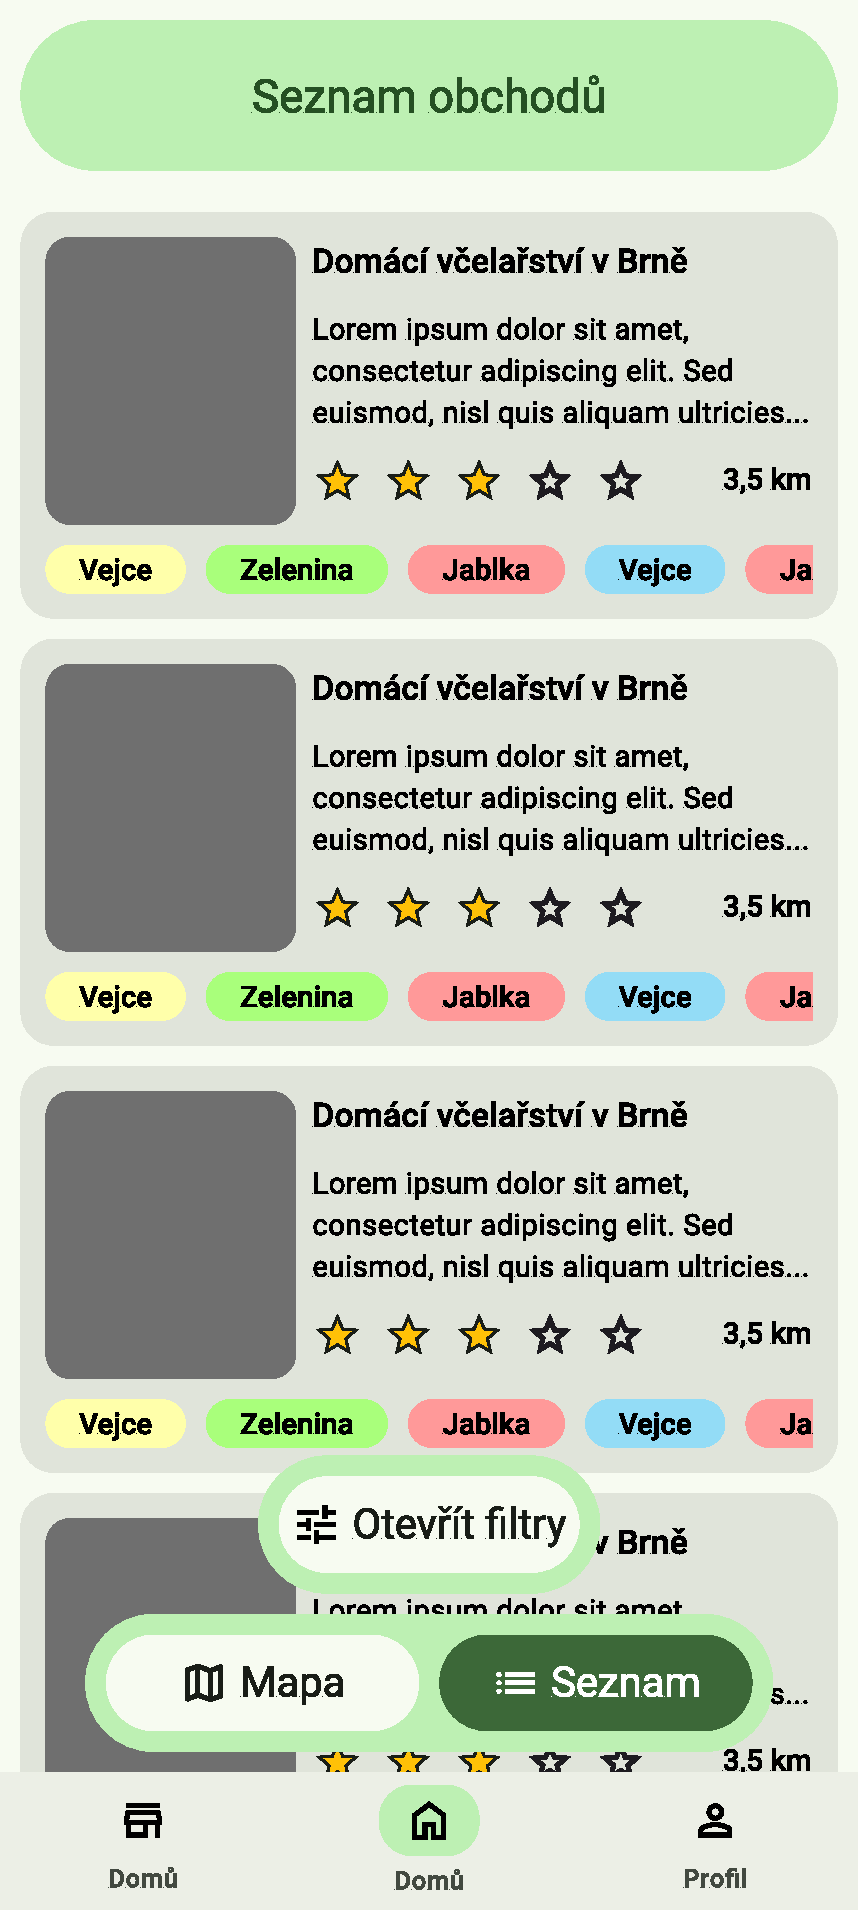
\includegraphics[width=\linewidth]{res/ui/list_view}
        \caption{Seznamové zobrazení obchodů}
        \label{fig:list-view}
    \end{subfigure}\hfill
    \begin{subfigure}[t]{0.24\textwidth}
        \centering
        \includegraphics[width=\linewidth]{res/ui/map_view_shop_detail}
        \caption{Detail obchodu v mapovém zobrazení}
        \label{fig:map-view-shop-detail}
    \end{subfigure}\hfill
    \begin{subfigure}[t]{0.24\textwidth}
        \centering
        \includegraphics[width=\linewidth]{res/ui/shop_detail}
        \caption{Detail obchodu v plném zobrazení}
        \label{fig:shop-detail}
    \end{subfigure}

    \caption{Přehled uživatelského rozhraní aplikace}
    \label{fig:ui-overview}
\end{figure}

\begin{figure}
    \centering
    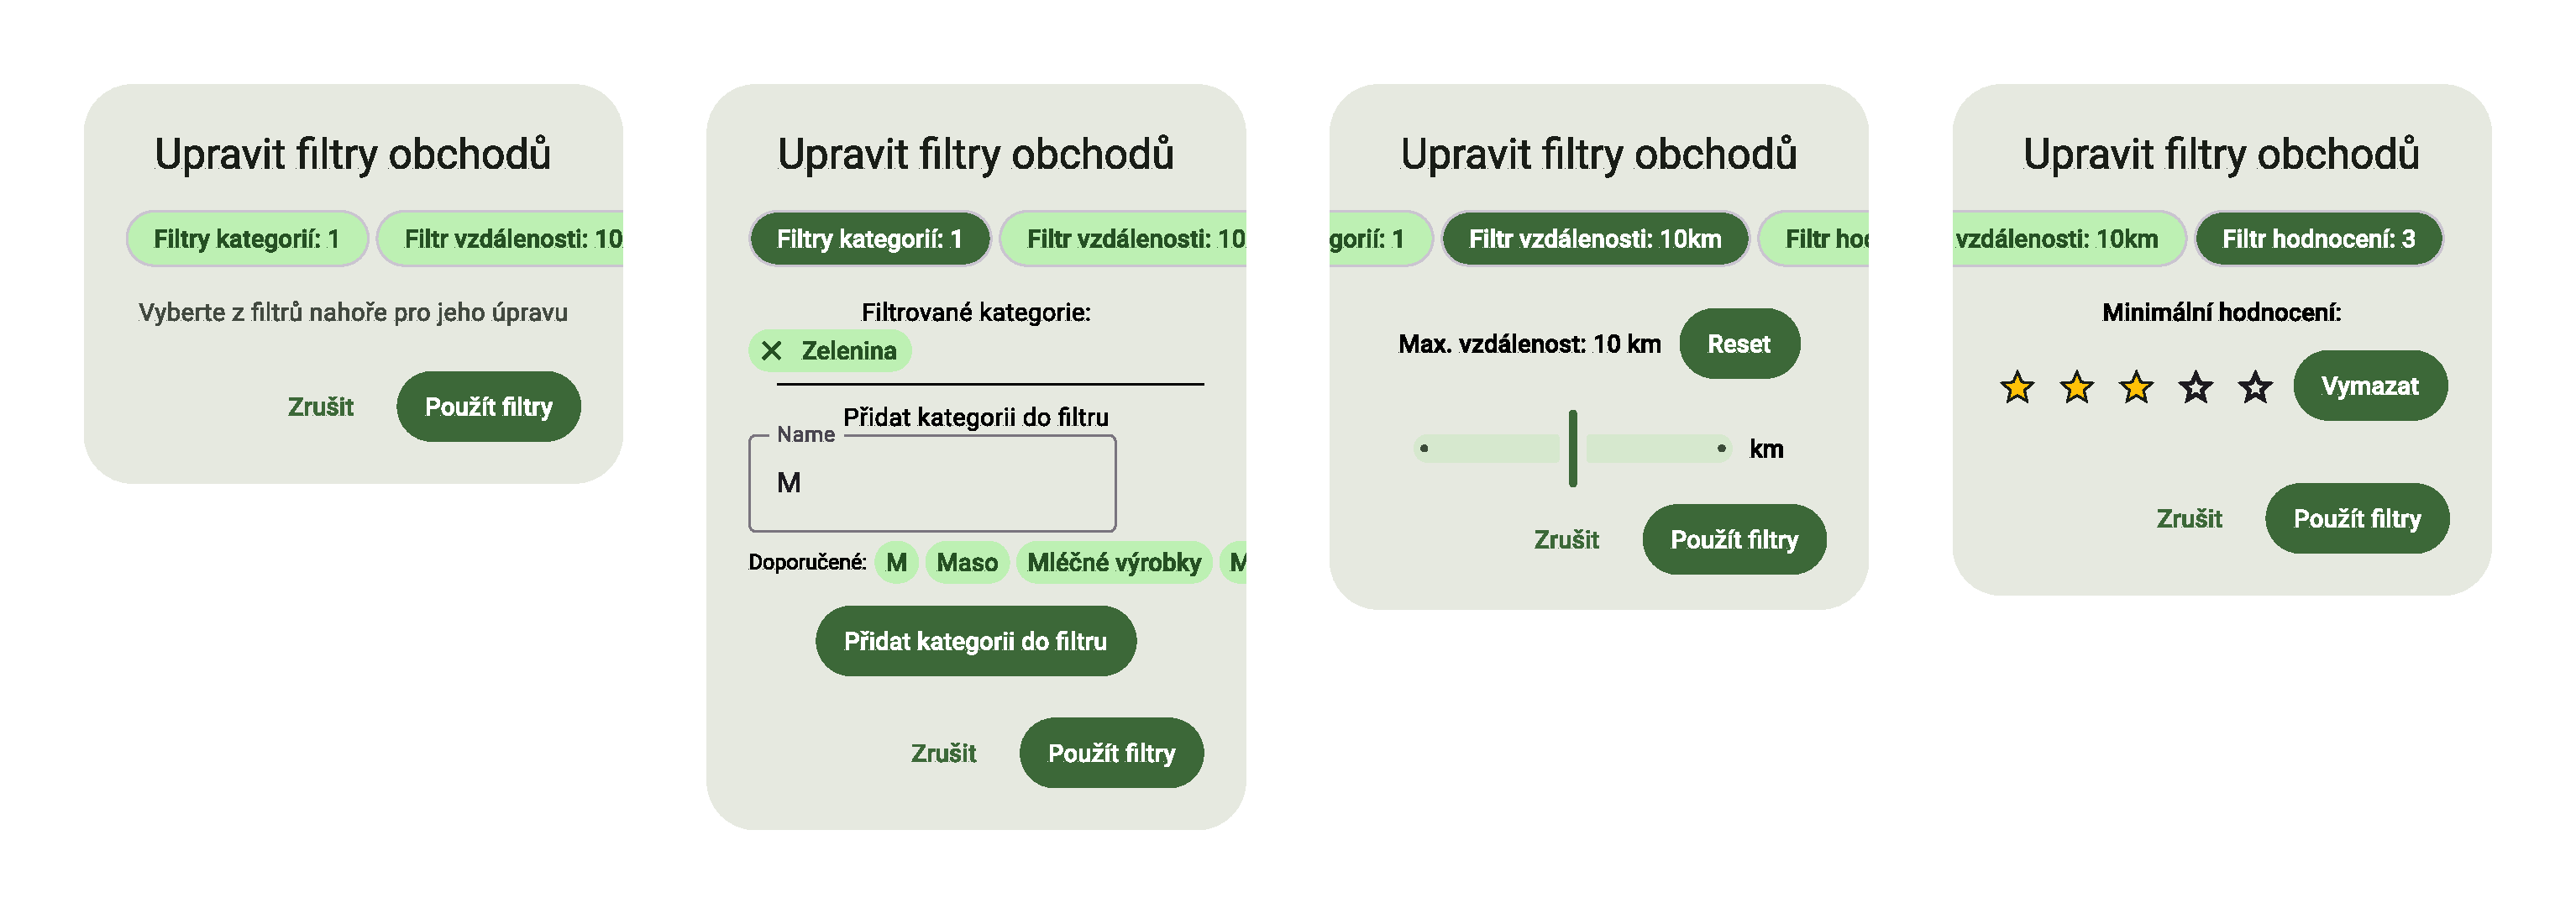
\includegraphics[width=\linewidth]{res/ui/filters}
    \caption{Dialog pro nastavení filtrů}
    \label{fig:filters}
\end{figure}

Ve spodní části základních obrazovek se nachází navigační lišta.
Díky ní může uživatel snadno navigovat mezi právě těmito základními obrazovkami aplikace.
První ikona v liště slouží pro navigaci na obrazovku se seznamem obchodů vytvořených uživatelem.
Tato ikona se v navigační liště zobrazuje pouze pokud je uživatel přihlášen.
Druhá ikona slouží pro navigaci na úvodní obrazovku s mapovým a seznamovým zobrazením obchodů.
Třetí ikona slouží pro navigaci na obrazovku profilu uživatele.
V případě, že je uživatel přihlášen, je na této obrazovce možné upravit osobní údaje.
V opačném případě se zobrazí přihlašovací obrazovka, kde se může uživatel přihlásit nebo zaregistrovat nový účet.

Na obrazovce profilu může uživatel upravit své osobní údaje, jak bylo specifikováno ve funkčních požadavcích.
Mezi tyto údaji patří jméno, kontaktní informace a profilový obrázek.
V případě profilového obrázku může uživatel buď nahrát obrázek ze svého zařízení, nebo přímo vyfotit nový obrázek pomocí fotoaparátu zařízení.
Uživatel se zde také může odhlásit z aplikace.

Na obrazovce \enquote{Moje obchody} má uživatel přehled o všech obchodech, které vytvořil.
Obchody jsou zobrazeny jako karty v seznamu, podobně jako v seznamovém zobrazení na úvodní obrazovce.
Každá karta má však navíc tlačítka pro úpravu a odstranění obchodu.
Po kliknutí na tlačítko pro úpravu se spustí proces úpravy obchodu a po kliknutí na tlačítko pro odstranění se daný obchod smaže.
K tomu se ve spodní části obrazovky nachází tlačítko pro vytvoření nového obchodu.
Po kliknutí na toto tlačítko se spustí proces vytváření nového obchodu.

Proces vytváření a úpravy obchodu je rozdělen do několika kroků a každý krok je zobrazen na samostatné obrazovce.
Uživatel může mezi těmito kroky libovolně navigovat pomocí dvou spodních tlačítek \enquote{Předchozí} a \enquote{Další}.

TODO: jednotlivé kroky\ldots - UI návrh done

%V posledním kroku se zobrazí shrnutí zadaných údajů před vytvořením obchodu a místo tlačítka \enquote{Další} se zobrazí tlačítko \enquote{Potvrdit}, které obchod vytvoří nebo upraví.


\section{Výběr technologií}
% Compose (vs Java/xml), Material 3, Firebase (vs Server Backend, vs Spring Server a proč jsem si to nevybral), Dokumentová databáze (vs SQL), BaaS, Serverless backend??
